% @author Sebastian Olsson
%
% Anv: 294 142 104
% Psw: 2nzp19
%
% quad-bild i team18/kivy/untitled.png
% activate-grej i program files/code laboratories/cl-eye platform sdk

\documentclass[a4paper,12pt]{article}
\usepackage[utf8]{inputenc}
\usepackage[swedish]{babel}
\usepackage[parfill]{parskip}
\usepackage{tikz}

\author{Sebastian Olsson}
\title{DD143X: Finalizing the architecture}
\date{17 april 2013}
\begin{document}
\maketitle
\begin{abstract}
    Mötesanteckningar från mötet 130417, 13.15-15.02.
\end{abstract}

\section{Mötet börjar}
Sebastian förklarar mötet öppnat.

Närvarande:
\begin{itemize}
\item Sebastian Olsson
\item Chjun-Chi Chiu
\item Kristoffer Hallqvist
\end{itemize}
Frånvarande:
\begin{itemize}
\item Dmitrij Lioubartsev
\item Andrew Saka
\item Jonatan Åkesson
\end{itemize}

Ordförande: Sebastian Olsson

Sekreterare: Sebastian Olsson

Mötesplats: Vid en bänk utanför Voljären.

\section{Föregående protokoll}
Referens: RADD Startup Phase.

\begin{enumerate}
\item Verkställd.
\item Verkställd. Dmitrij lade upp ett bidrag i vår repository.
\item Verkställd. Som resultat har vi kommit fram till en ny arkitektur. Se Beslut.
\item Verkställd.
\end{enumerate}

\section{Diskussionsteman}
\begin{itemize}
\item Fyra kameror
\item Scroll/pinch-funktionalitet
\item 1 vs. 2 vs. 3 Kivy-sessions
\item Datacentrerad arkitektur
\item Testning
\item GUI:t
\item Skript för kommandon
\item RADD: arbetsuppdelning och arbetstider
\end{itemize}

\section{TODO}
\begin{itemize}
\item Gör det möjligt att använda GUI:t samtidigt som man styr Windows.
\item Gör det möjligt att framställa egna gester (från GUI:t?).
\item Gör det möjligt att definiera egna commands via skript (från GUI:t).
\item Gör det enkelt att sätta sig in i hur man skriver commands: skriv en dokumentation
(manual?) för vårt skriptspråk och gärna en modul som CommandHandler importerar som
innehåller metoder för alla kommandon.
\item Skriv en manual (basic-krav).
\item Skriv RADD:n.
\item Mycket mer som sekreteraren inte kommer på på rak arm.
\end{itemize}

\section{Beslut}
\begin{itemize}
\item Jonatan kontaktar Henrik om en experimentomgång nästa vecka.
\item Arkitekturen revideras något. Nu är det tänkt att GestureHandlern och GUI:t är starkt
sammankopplade (t.o.m. samma modul?) och att GUI:t är fullständigt geststyrt. Detta skiljer sig
från förut, då det var tänkt att GUI:t och GestureHandlern styrdes av två olika
TUIO-strömmar/fönster.
\end{itemize}

\begin{figure}
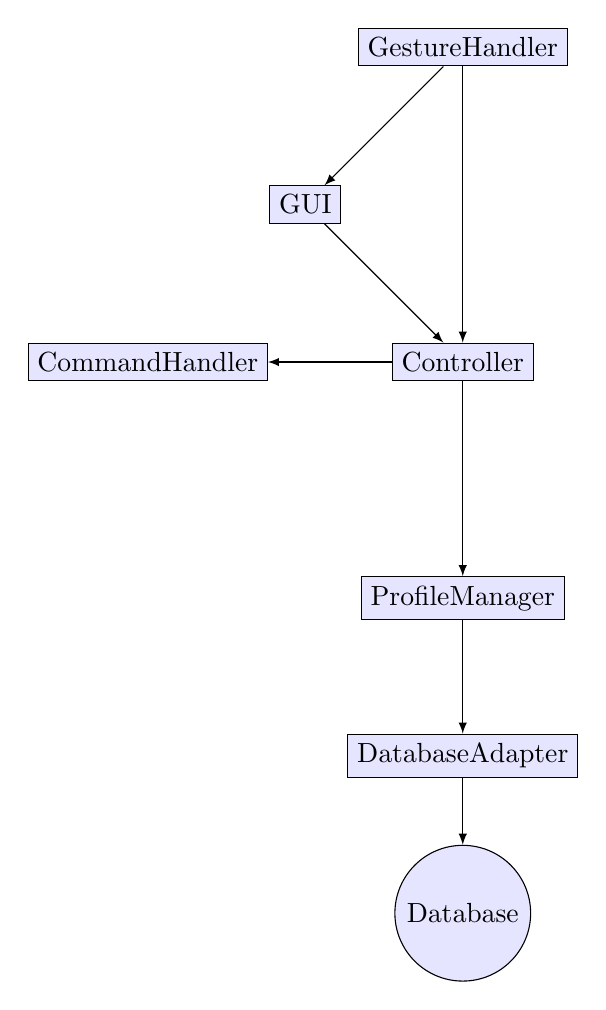
\begin{tikzpicture}
\node[rectangle,draw,fill=blue!10] (v3) at (0,0) {Controller};
\node[rectangle,draw,fill=blue!10] (v2) at (-2,2) {GUI};
\node[rectangle,draw,fill=blue!10] (v5) at (-4,0) {CommandHandler};
\node[rectangle,draw,fill=blue!10] (v1) at (0,4) {GestureHandler};
\node[rectangle,draw,fill=blue!10] (v4) at (0,-3) {ProfileManager};
\node[circle,draw,fill=blue!10] (v7) at (0,-7) {Database};
\node[rectangle,draw,fill=blue!10] (v6) at (0,-5) {DatabaseAdapter};
\draw[-latex]  (v1) edge (v2);
\draw[-latex]  (v1) edge (v3);
\draw[-latex]  (v2) edge (v3);
\draw[-latex]  (v3) edge (v4);
\draw[-latex]  (v3) edge (v5);
\draw[-latex]  (v4) edge (v6);
\draw[-latex]  (v6) edge (v7);
\end{tikzpicture}
\caption{Den nya arkitekturen?}
\end{figure}

\section{Nästa möte}
Vid experimentomgången nästa vecka, i Voljären.
\end{document}
